\documentclass{../myclass}
\usepackage[polish]{babel}

\begin{document}

\begin{center}
    \Large \textbf{Laboratorium 3.}\\
    \large
    \textsc{Rekurencyjna kompresja macierzy}\\
    \normalsize
    Bartosz Hanc
\end{center}

\section{Wstęp}

Celem ćwiczenia było napisanie rekurencyjnej kompresji macierzy z wykorzystaniem algorytmu
częściowego SVD oraz wizualizacji uzyskiwanych w tej procedurze macierzy hierarchicznych. Dodatkowo
zmierzono czas kompresji macierzy oraz błąd względny między macierzą wejściową, a macierzą uzyskaną
po dekompresji dla różnych minimalnych wartości osobliwych i maksymalnego rank.

\section{Kod rozwiązania}

Poniżej zamieszczono kod rozwiązania w języku Python. Węzły drzewa były reprezentowane jako
struktury \pythoninline{Node}, których definicję zawarto poniżej. Funkcja
\pythoninline{CreateTree()} odpowiada za stworzenie drzewa kompresji, a
\pythoninline{CompressMatrix()} za skompresowanie liścia korzystając z algorytmu SVD.

\begin{python}
class Node:
    def __init__(self, rank=None, side=None, sMin=None, 
                tMin=None, U=None, V=None, D=None):
        self.next: list[Node] = []
        self.sMin: int = sMin
        self.tMin: int = tMin
        self.side: int = side
        self.rank: int = rank
        self.U: np.ndarray[float] = U
        self.D: np.ndarray[float] = D
        self.V: np.ndarray[float] = V
\end{python}
\begin{python}
def CompressMatrix(A, U, D, V: np.ndarray[float], r, sMin, tMin):
    if np.allclose(A, np.zeros(A.shape)):
        return Node(rank=0, side=A.shape[0], sMin=sMin, tMin=tMin)

    return Node( rank=r, side=A.shape[0], sMin=sMin, tMin=tMin,
            U=U[:, :r], D=D[:r], V=V[:r, :])
\end{python}
\newpage
\begin{python}
def CreateTree(A, r, eps, sMin = 0, tMin = 0):
    n = A.shape[0]
    U, D, V = randomized_svd(A, r + 1) # from sklearn.utils.extmath
    if len(D) <= r or D[r] < eps:
        v = CompressMatrix(A, U, D, V, len(D), sMin, tMin)
    else:
        v = Node(rank=None, side=n, sMin=sMin, tMin=tMin)
        v.next.append(CreateTree(A[: n // 2, : n // 2], 
                        r, eps, sMin, tMin))

        v.next.append(CreateTree(A[n // 2 :, : n // 2], 
                        r, eps, sMin + n // 2, tMin))

        v.next.append(CreateTree(A[: n // 2, n // 2 :], 
                        r, eps, sMin, tMin + n // 2))

        v.next.append(CreateTree(A[n // 2 :, n // 2 :], 
                        r, eps, sMin + n // 2, tMin + n // 2))
    return v
\end{python}

Funkcja \pythoninline{Decompress()} odpowiada za dekompresje macierzy z uzyskanej struktury
drzewiastej.

\begin{python}
def Decompress(root: Node):
    n = root.side
    A = np.zeros((n, n))

    def DecompressRecursive(root: Node):
        nonlocal A
        if root.rank is None:  # Not a leaf -> pass
            pass
        elif root.rank == 0:  # Leaf with all 0s -> pass
            pass
        elif root.rank > 0:
            s, t, side = root.sMin, root.tMin, root.side
            U, D, V = root.U, np.diag(root.D), root.V
            A[s : s + side, t : t + side] = U @ D @ V

        for node in root.next:
            DecompressRecursive(node)

    DecompressRecursive(root)
    return A
\end{python}
\newpage
Analogicznie została zaimplementowana funkcja służąca do wizualizacji.
\begin{python}
def DrawTree(root: Node):
    n = root.side
    fig, ax = plt.subplots()
    ax.set_aspect("equal", "box")
    ax.set_xlim(0, n)
    ax.set_ylim(0, n)

    def DrawTreeRecursive(root: Node):
        nonlocal ax

        if root.rank is None:  # Not a leaf -> draw grid lines
            x, y, d = root.sMin, root.tMin, root.side // 2
            ax.plot((x, x + 2 * d), (y + d, y + d), color="k", lw=0.6)
            ax.plot((x + d, x + d), (y, y + 2 * d), color="k", lw=0.6)

        elif root.rank > 0:  # Leaf with SVD -> fill block
            x, y, d = root.sMin, root.tMin + root.side, root.side
            lw = root.side / (6 * root.rank)
            for i in range(root.rank):
                ax.fill([x, x + d, x + d, x], 
                        [y, y, y - (i + 1) * lw, y - (i + 1) * lw], 
                        color="k")
                ax.fill([x, x + (i + 1) * lw, x + (i + 1) * lw, x], 
                        [y, y, y - d, y - d], 
                        color="k")

        elif root.rank == 0:  # Leaf with all 0s -> pass
            pass

        for node in root.next:
            DrawTreeRecursive(node)

    DrawTreeRecursive(root)
    fig.show()
\end{python}
\newpage

\section{Wyniki}

Wylosowano macierze wymiarów \(512 \times 512\) zawierające odpowiednio 1, 2, 5, 10, i 20 procent
elementów niezerowych. Dla każdej z macierzy wykonano wykres wartości osobliwych, który zamieszczono
poniżej.

\begin{figure}[ht]
    \centering
    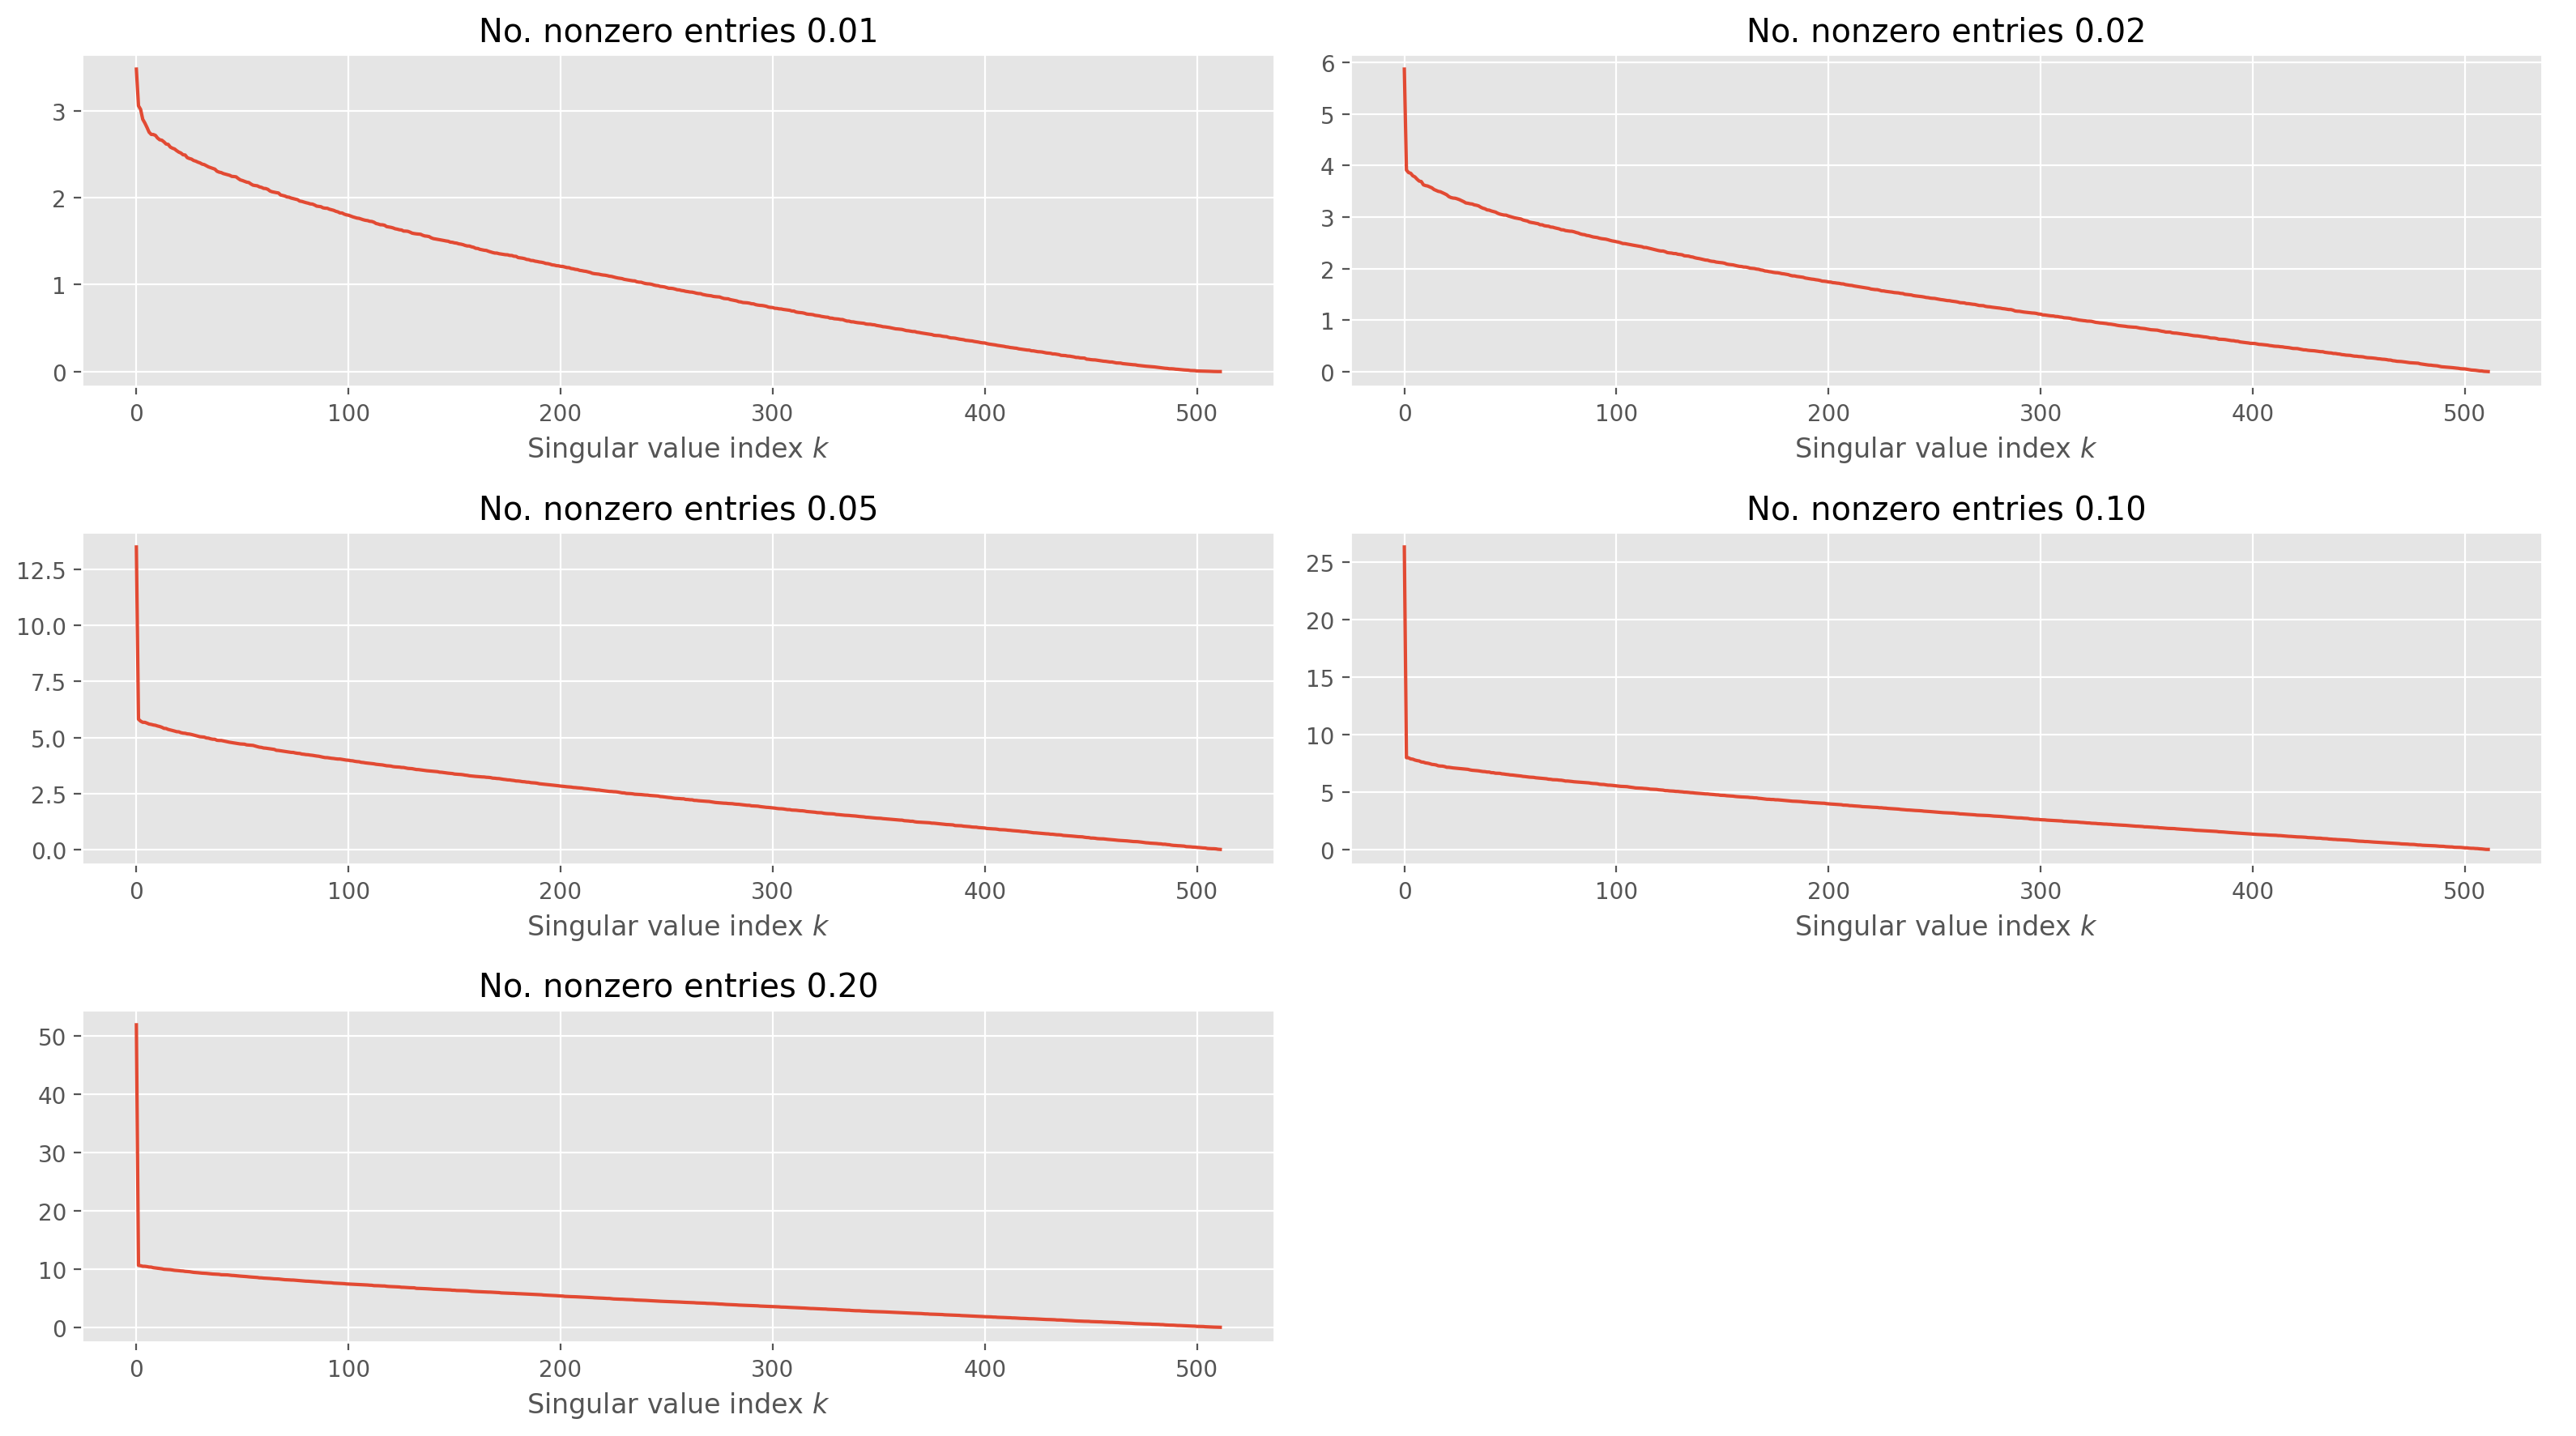
\includegraphics[width=0.95\textwidth]{singular_values.png}
    \caption{Wykres wartości osobliwych dla różnych losowych macierzy}    
\end{figure}

Następnie dla wylosowanych macierzy oraz parametrów \(r\) (maksymalny rank) oraz \(\epsilon\)
(minimalna wartość osobliwa) ze zbiorów odpowiednio \(\{1,4\}\) i \(\{\sigma_2, \sigma_{2^{1023}},
\sigma{2^{1024}}\}\) wykonano kompresje macierzy oraz zwizualizowano powstałe w ten sposób macierze
hierarchiczne. Dodatkowo zmierzono czasy kompresji. Uzyskane wyniki zawarto poniżej. W Tabeli
\ref{Tab:1} zamieszczono zmierzone czasy kompresji oraz obliczony błąd średniokwadratowy. Względny
błąd średniokwadratowy został obliczony jako stosunek
\begin{equation}
    \frac{\norm{\oper{A} - \tilde{\oper{A}}}}{\norm{\oper{A}}} = \sqrt{\frac{\sum_{i,j}(A_{ij} - \tilde{A}_{ij})^2}{\sum_{i,j}A_{ij}^2}}\,,
\end{equation}
gdzie \(\oper{A}\) jest macierzą przed kompresją, a \(\tilde{\oper{A}}\) jest macierzą \(\oper{A}\)
po dekompresji ze struktury macierzy hierarchicznej. Na Rysunku \ref{Fig:1} zamieszczono również
wizualizacje otrzymanych macierzy hierarchicznych.

\begin{table}[ht]
    \centering
    \begin{tabular}{ccccc}
    \hline
    \multicolumn{1}{|c|}{\begin{tabular}[c]{@{}c@{}}Proc. zerowych\\ wartości\end{tabular}} &
    \multicolumn{1}{c|}{\(r\)} & \multicolumn{1}{c|}{\begin{tabular}[c]{@{}c@{}}indeks \\
    \(\sigma_k\)\end{tabular}} & \multicolumn{1}{c|}{Czas {[}s{]}} &
    \multicolumn{1}{c|}{\begin{tabular}[c]{@{}c@{}}Błąd\\ średniokwadratowy\end{tabular}} \\ \hline
    \multicolumn{1}{l}{}                                                                    &
    \multicolumn{1}{l}{}       & \multicolumn{1}{l}{}
    & \multicolumn{1}{l}{}              & \multicolumn{1}{l}{}
    \\ \hline
    \multicolumn{1}{|c|}{0.99}                                                              &
    \multicolumn{1}{c|}{1}     & \multicolumn{1}{c|}{512}
    & \multicolumn{1}{c|}{1.07}         & \multicolumn{1}{c|}{1.45e-16}
    \\ \hline
    \multicolumn{1}{|c|}{0.99}                                                              &
    \multicolumn{1}{c|}{1}     & \multicolumn{1}{c|}{2}
    & \multicolumn{1}{c|}{0.01}         & \multicolumn{1}{c|}{9.88e-01}
    \\ \hline
    \multicolumn{1}{|c|}{0.99}                                                              &
    \multicolumn{1}{c|}{1}     & \multicolumn{1}{c|}{256}
    & \multicolumn{1}{c|}{0.26}         & \multicolumn{1}{c|}{5.60e-01}
    \\ \hline
    \multicolumn{1}{|c|}{0.99}                                                              &
    \multicolumn{1}{c|}{4}     & \multicolumn{1}{c|}{512}
    & \multicolumn{1}{c|}{0.53}         & \multicolumn{1}{c|}{7.35e-16}
    \\ \hline
    \multicolumn{1}{|c|}{0.99}                                                              &
    \multicolumn{1}{c|}{4}     & \multicolumn{1}{c|}{2}
    & \multicolumn{1}{c|}{0.01}         & \multicolumn{1}{c|}{9.74e-01}
    \\ \hline
    \multicolumn{1}{|c|}{0.99}                                                              &
    \multicolumn{1}{c|}{4}     & \multicolumn{1}{c|}{256}
    & \multicolumn{1}{c|}{0.11}         & \multicolumn{1}{c|}{5.02e-01}
    \\ \hline
    \multicolumn{1}{|c|}{0.98}                                                              &
    \multicolumn{1}{c|}{1}     & \multicolumn{1}{c|}{512}
    & \multicolumn{1}{c|}{1.89}         & \multicolumn{1}{c|}{1.50e-16}
    \\ \hline
    \multicolumn{1}{|c|}{0.98}                                                              &
    \multicolumn{1}{c|}{1}     & \multicolumn{1}{c|}{2}
    & \multicolumn{1}{c|}{0.01}         & \multicolumn{1}{c|}{9.86e-01}
    \\ \hline
    \multicolumn{1}{|c|}{0.98}                                                              &
    \multicolumn{1}{c|}{1}     & \multicolumn{1}{c|}{256}
    & \multicolumn{1}{c|}{0.17}         & \multicolumn{1}{c|}{7.78e-01}
    \\ \hline
    \multicolumn{1}{|c|}{0.98}                                                              &
    \multicolumn{1}{c|}{4}     & \multicolumn{1}{c|}{512}
    & \multicolumn{1}{c|}{0.69}         & \multicolumn{1}{c|}{7.58e-16}
    \\ \hline
    \multicolumn{1}{|c|}{0.98}                                                              &
    \multicolumn{1}{c|}{4}     & \multicolumn{1}{c|}{2}
    & \multicolumn{1}{c|}{0.01}         & \multicolumn{1}{c|}{9.73e-01}
    \\ \hline
    \multicolumn{1}{|c|}{0.98}                                                              &
    \multicolumn{1}{c|}{4}     & \multicolumn{1}{c|}{256}
    & \multicolumn{1}{c|}{0.09}         & \multicolumn{1}{c|}{7.39e-01}
    \\ \hline
    \multicolumn{1}{|c|}{0.95}                                                              &
    \multicolumn{1}{c|}{1}     & \multicolumn{1}{c|}{512}
    & \multicolumn{1}{c|}{3.77}         & \multicolumn{1}{c|}{1.51e-16}
    \\ \hline
    \multicolumn{1}{|c|}{0.95}                                                              &
    \multicolumn{1}{c|}{1}     & \multicolumn{1}{c|}{2}
    & \multicolumn{1}{c|}{0.01}         & \multicolumn{1}{c|}{9.75e-01}
    \\ \hline
    \multicolumn{1}{|c|}{0.95}                                                              &
    \multicolumn{1}{c|}{1}     & \multicolumn{1}{c|}{256}
    & \multicolumn{1}{c|}{0.09}         & \multicolumn{1}{c|}{8.97e-01}
    \\ \hline
    \multicolumn{1}{|c|}{0.95}                                                              &
    \multicolumn{1}{c|}{4}     & \multicolumn{1}{c|}{512}
    & \multicolumn{1}{c|}{1.18}         & \multicolumn{1}{c|}{8.55e-16}
    \\ \hline
    \multicolumn{1}{|c|}{0.95}                                                              &
    \multicolumn{1}{c|}{4}     & \multicolumn{1}{c|}{2}
    & \multicolumn{1}{c|}{0.01}         & \multicolumn{1}{c|}{9.64e-01}
    \\ \hline
    \multicolumn{1}{|c|}{0.95}                                                              &
    \multicolumn{1}{c|}{4}     & \multicolumn{1}{c|}{256}
    & \multicolumn{1}{c|}{0.08}         & \multicolumn{1}{c|}{8.17e-01}
    \\ \hline
    \multicolumn{1}{|c|}{0.90}                                                              &
    \multicolumn{1}{c|}{1}     & \multicolumn{1}{c|}{512}
    & \multicolumn{1}{c|}{6.50}         & \multicolumn{1}{c|}{1.54e-16}
    \\ \hline
    \multicolumn{1}{|c|}{0.90}                                                              &
    \multicolumn{1}{c|}{1}     & \multicolumn{1}{c|}{2}
    & \multicolumn{1}{c|}{0.02}         & \multicolumn{1}{c|}{9.56e-01}
    \\ \hline
    \multicolumn{1}{|c|}{0.90}                                                              &
    \multicolumn{1}{c|}{1}     & \multicolumn{1}{c|}{256}
    & \multicolumn{1}{c|}{0.07}         & \multicolumn{1}{c|}{9.06e-01}
    \\ \hline
    \multicolumn{1}{|c|}{0.90}                                                              &
    \multicolumn{1}{c|}{4}     & \multicolumn{1}{c|}{512}
    & \multicolumn{1}{c|}{1.83}         & \multicolumn{1}{c|}{9.17e-16}
    \\ \hline
    \multicolumn{1}{|c|}{0.90}                                                              &
    \multicolumn{1}{c|}{4}     & \multicolumn{1}{c|}{2}
    & \multicolumn{1}{c|}{0.01}         & \multicolumn{1}{c|}{9.45e-01}
    \\ \hline
    \multicolumn{1}{|c|}{0.90}                                                              &
    \multicolumn{1}{c|}{4}     & \multicolumn{1}{c|}{256}
    & \multicolumn{1}{c|}{0.07}         & \multicolumn{1}{c|}{8.21e-01}
    \\ \hline
    \multicolumn{1}{|c|}{0.80}                                                              &
    \multicolumn{1}{c|}{1}     & \multicolumn{1}{c|}{512}
    & \multicolumn{1}{c|}{10.45}        & \multicolumn{1}{c|}{1.60e-16}
    \\ \hline
    \multicolumn{1}{|c|}{0.80}                                                              &
    \multicolumn{1}{c|}{1}     & \multicolumn{1}{c|}{2}
    & \multicolumn{1}{c|}{0.01}         & \multicolumn{1}{c|}{9.17e-01}
    \\ \hline
    \multicolumn{1}{|c|}{0.80}                                                              &
    \multicolumn{1}{c|}{1}     & \multicolumn{1}{c|}{256}
    & \multicolumn{1}{c|}{0.07}         & \multicolumn{1}{c|}{8.77e-01}
    \\ \hline
    \multicolumn{1}{|c|}{0.80}                                                              &
    \multicolumn{1}{c|}{4}     & \multicolumn{1}{c|}{512}
    & \multicolumn{1}{c|}{3.03}         & \multicolumn{1}{c|}{7.60e-16}
    \\ \hline
    \multicolumn{1}{|c|}{0.80}                                                              &
    \multicolumn{1}{c|}{4}     & \multicolumn{1}{c|}{2}
    & \multicolumn{1}{c|}{0.02}         & \multicolumn{1}{c|}{9.06e-01}
    \\ \hline
    \multicolumn{1}{|c|}{0.80}                                                              &
    \multicolumn{1}{c|}{4}     & \multicolumn{1}{c|}{256}
    & \multicolumn{1}{c|}{0.08}         & \multicolumn{1}{c|}{7.99e-01}
    \\ \hline
    \end{tabular}
    \caption{Tabela porównująca czas kompresji i błąd dla różnych macierzy i parametrów \(r\), \(\epsilon\)}
    \label{Tab:1}
    \end{table}


\begin{figure}
    \centering
    \begin{subfigure}[b]{0.45\textwidth}
        \centering
        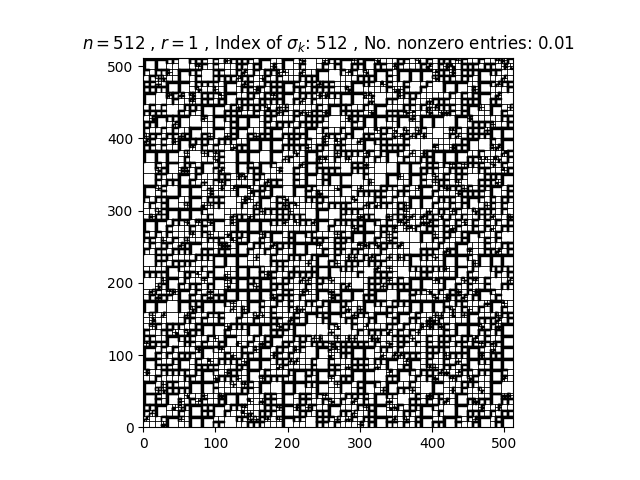
\includegraphics[width=\textwidth]{hm_0.01_1_512.png}
    \end{subfigure}
    \hfill
    \begin{subfigure}[b]{0.45\textwidth}
        \centering
        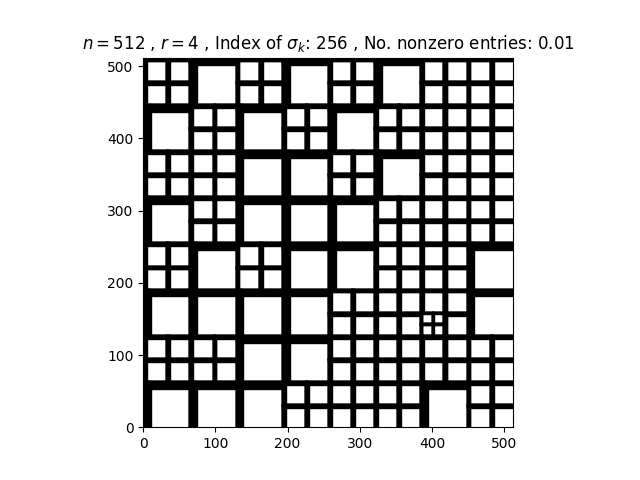
\includegraphics[width=\textwidth]{hm_0.01_4_256.png}
    \end{subfigure}
    \vfill
    \centering
    \begin{subfigure}[b]{0.45\textwidth}
        \centering
        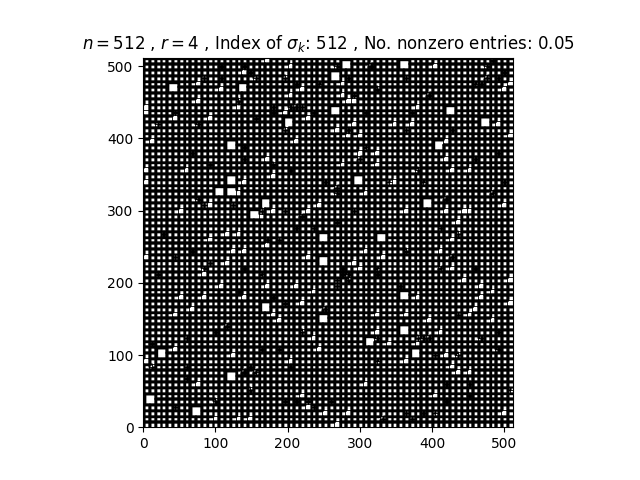
\includegraphics[width=\textwidth]{hm_0.05_4_512.png}
    \end{subfigure}
    \hfill
    \begin{subfigure}[b]{0.45\textwidth}
        \centering
        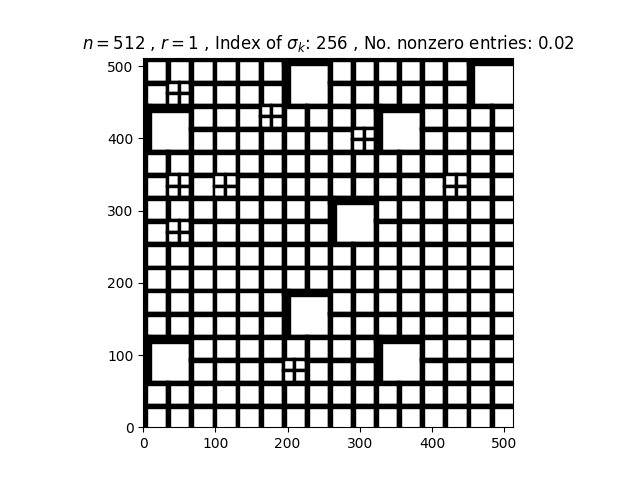
\includegraphics[width=\textwidth]{hm_0.02_1_256.png}
    \end{subfigure}
    \vfill
    \centering
    \begin{subfigure}[b]{0.45\textwidth}
        \centering
        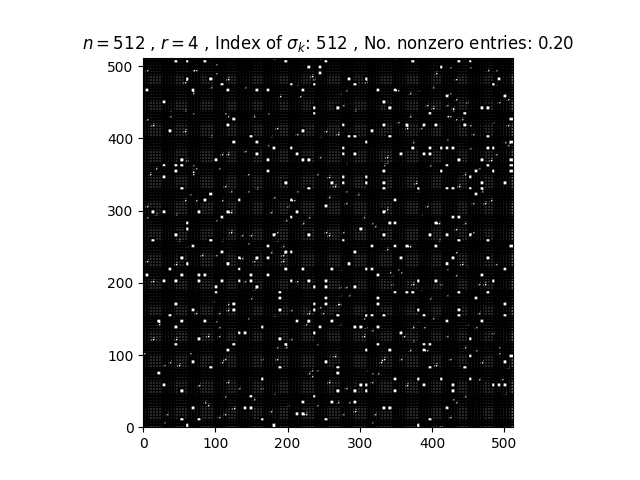
\includegraphics[width=\textwidth]{hm_0.20_4_512.png}
    \end{subfigure}
    \hfill
    \begin{subfigure}[b]{0.45\textwidth}
        \centering
        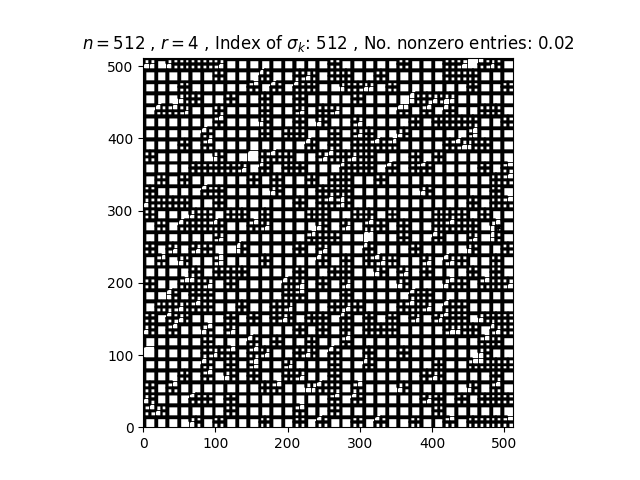
\includegraphics[width=\textwidth]{hm_0.02_4_512.png}
    \end{subfigure}
    \caption{Wizualizacje uzyskanych macierzy hierarchicznych}
    \label{Fig:1}
\end{figure}

\end{document}
